% Copyright 2018-2021 Melvin Eloy Irizarry-Gelpí
\setcounter{chapter}{3}
\chapter{Faraday's Law of Induction}
%
In this experiment you will learn about Faraday's law of induction and a relationship between electric and magnetic phenomena.
%
\section{Preliminary}
%
Faraday's law of induction is a statement relating an \textbf{electric} phenomenon to a \textbf{magnetic} phenomenon. It states that a certain amount of \textbf{voltage} $\mathcal{E}$ is equal to the negative \textbf{rate of change of the magnetic flux} $\Phi_{B}$ with time:
\begin{equation}
	\mathcal{E} = -\frac{\Delta \Phi_{B}}{\Delta t}
	\label{eq.04.faradays.law}
\end{equation}
Here $\mathcal{E}$ is known as the \textbf{electro-motive force} or EMF. Although ``force'' is part of its name, an EMF quantity has nothing to do with force (which is measured in newtons): an EMF quantity has units of volts.
%
\subsection{Magnetic flux and its rate of change}
%
The \textbf{magnetic flux} is defined as the product of the amount of \textbf{magnetic field} $B$ and the amount of \textbf{area} $a$ in a surface where the magnetic field lines pass through:
\begin{equation}
	\Phi_{B} = B a
\end{equation}
The \textbf{SI unit} for magnetic field is the \textbf{tesla} (T). The \textbf{SI unit} for area is the square meter (m$^{2}$). Thus, magnetic flux is measured in units of T {\textperiodcentered} m\textsuperscript{2}.

A non-zero EMF $\mathcal{E}$ requires the magnetic flux $\Phi_{B}$ to change with time. In this experiment you are going to keep the \textbf{area fixed} and let the \textbf{magnetic field change with time}. In this setting, the rate of change of the magnetic flux with time is proportional to the rate of change of the magnetic field with time:
\begin{align}
	\Phi_{B} = B a && \Longrightarrow && \frac{\Delta \Phi_{B}}{\Delta t} = \left(\frac{\Delta B}{\Delta t}\right) a
	\label{eq.04.flux.rate}
\end{align}
The rate of change of magnetic flux is measured in units of T {\textperiodcentered} m\textsuperscript{2}/s. But according to Faraday's law, these units are the same as the units for EMF (volts), so you must have the equivalence:
\begin{equation}
	1 \ \text{V} = 1 \ \text{T {\textperiodcentered} m\textsuperscript{2}/s}
\end{equation}
This allows you to express the tesla unit in terms of volts, meters, and seconds:
\begin{equation}
	1 \ \text{T} = 1 \ \text{V {\textperiodcentered} s/m\textsuperscript{2}}
\end{equation}
%
\subsection{Producing the magnetic field}
%
Wires with electric current produce magnetic fields. You are going to use a particular wire called a \textbf{solenoid coil}. The \textbf{magnetic field} $B$ inside the cylindrical space of a solenoid coil is (almost) uniform and the amount of field is directly proportional to the amount of current $I$ flowing through the coil:
\begin{equation}
	B = \left(\frac{\mu_{0} N_{1}}{L}\right) I
	\label{eq.04.B.coil}
\end{equation}
Here
\begin{itemize}
	\item $B$ is the amount of \textbf{magnetic field} (unit: T)
	\item $\mu_{0} = 4 \pi \times 10^{-7}$ T {\textperiodcentered} m/A  is a universal physical \textbf{constant}
	\item $N_{1}$ is the \textbf{number of turns} in the (primary) coil (no units)
	\item $L$ is the \textbf{length} of the (primary) coil (unit: m)
	\item $I$ is the amount of \textbf{electric current} through the (primary) coil (unit: A)
\end{itemize}
For a given coil you are going to keep the \textbf{number of turns fixed}, and the \textbf{length fixed}, but you are going to use a \textbf{current that changes with time}. In this case, the rate of change of the magnetic field with time is proportional to the rate of change of the current with time:
\begin{align}
	B = \left(\frac{\mu_{0} N_{1}}{L}\right) I && \Longrightarrow && \frac{\Delta B}{\Delta t} = \left( \frac{\mu_{0} N_{1}}{L} \right) \frac{\Delta I}{\Delta t}
	\label{eq.04.B.rate}
\end{align}
Using Equation (\ref{eq.04.B.rate}) in Equation (\ref{eq.04.flux.rate}) gives
\begin{equation}
	\frac{\Delta \Phi_{B}}{\Delta t} = \left( \frac{\mu_{0} N_{1} a}{L} \right) \frac{\Delta I}{\Delta t}
\end{equation}
Thus, according to Faraday's law, for a solenoid coil you should have
\begin{equation}
	\mathcal{E} = -\left( \frac{\mu_{0} N_{1} a}{L} \right) \frac{\Delta I}{\Delta t}
	\label{eq.04.emf.solenoid}
\end{equation}
That is, the EMF associated with the area $a$ is proportional to the rate of change of the electric current with respect to time.
%
\section{Experiment}
%
The overall goal of the experiment is to check that the EMF behaves like the rate of change of the electric current. To do this you need to measure the EMF voltage and the current. From the current you can estimate the rate of change and confirm that it agrees with the EMF data.

You are going to look at \textbf{five ways for the current to change with time}:
\begin{enumerate}
	\item \textbf{Sinusoidal}: current will change according to a \textbf{sine or cosine} profile.
	\item \textbf{Square}: current will stay almost \textbf{constant}, but the \textbf{sign changes}.
	\item \textbf{Triangular}: current will increase \textbf{linearly}, then decrease \textbf{linearly}.
	\item \textbf{Ramp-up}: current will \textbf{increase linearly}, then \textbf{abruptly drop} to its base value.
	\item \textbf{Ramp-down}: current will \textbf{decrease linearly}, then \textbf{abruptly rise} to its base value.
\end{enumerate}
Each profile for the current leads to different results for the induced EMF.
%
\subsection{Rates of Change}
%
Here is a quick review of rates of change.
%
\subsubsection{Constant Quantity}
%
The rate of change of a \textbf{constant quantity} is \textbf{zero}. That is, if the quantity is not changing, then no amount is being gained or lost.
%
\subsubsection{Quantity Increasing Linearly}
%
The rate of change of a \textbf{quantity that increases linearly with time} is a \textbf{constant}. Increasing linearly is the same as being proportional to time. This means that the slope is constant. Moreover, since the quantity is increasing, the \textbf{slope is positive}.
%
\subsubsection{Quantity Decreasing Linearly}
%
The rate of change of a \textbf{quantity that decreases linearly with time} is a \textbf{constant}. Decreasing linearly is the same as being proportional to time. This means that the slope is constant. However, since the quantity is decreasing, the \textbf{slope is negative}.
%
\subsubsection{Sinusoidal Change}
%
The rate of change of the \textbf{sine function} is a cosine function:
\begin{equation}
	\frac{\Delta \sin(t)}{\Delta t} = \cos(t)
\end{equation}
Similarly, the rate of change of the \textbf{cosine function} is proportional to a sine function:
\begin{equation}
	\frac{\Delta \cos(t)}{\Delta t} = -\sin(t)
\end{equation}
Here the sign is not important. What is important is to remember that sine and cosine are very similar functions and that a cosine is the same as a sine function shifted by 90 deg (or $\pi/2$ rad):
\begin{align}
	\cos(t) = \sin(t + 90\text{\textdegree}), && \sin(t) = \cos(t - 90\text{\textdegree})
\end{align}
Thus, if the quantity is sinusoidal, then the rate of change will also be sinusoidal but shifted by 90 deg. In particular, when $\sin(t)$ is at a peak or valley, then $\cos(t)$ is crossing the horizontal axis (i.e. close to zero), and when $\sin(t)$ is crossing the horizontal axis (i.e. close to zero), then $\cos(t)$ is either at a valley or a peak.
%
\subsection{Solenoid Coils}
%
You are going to use two solenoid coils. The smaller one fits inside the larger one. The smaller one is called the \textbf{secondary coil}. This is the coil used to measure the EMF value. The larger coil is called the \textbf{primary coil}. This coil is the one with the current and the one that produces the magnetic field.

The \textbf{primary coil} has a length of 10 cm and 3300 turns. Thus,
\begin{align}
	L = 10 \ \text{cm} = 0.1 \ \text{m,} && N_{1} = 3300
\end{align}
The \textbf{secondary coil} has 150 turns and an outer diameter of 1.8 cm. The inner diameter I measured it to be close to 1.1 cm. The average of these two diameters correspond to the diameter half-way between these two. This average is 1.45 cm. Since the wire was very thick, I think it is more accurate to use the average of the diameters to calculate the area of each loop. Thus,
\begin{align}
	d = 1.45 \ \text{cm} = 0.0145 \ \text{m,} && N_{2} = 150
\end{align}
The area enclosed by a circular loop with diameter $d$ is given by
\begin{equation}
	a_{\text{loop}} = \frac{1}{4} \pi d^{2} = \frac{1}{4} \pi \left(0.0145 \ \text{m}\right)^2 = 1.65 \times 10^{-4} \ \text{m\textsuperscript{2}}
\end{equation}
This is the amount of \textbf{area-per-loop} in the secondary coil. The \textbf{total amount of area} $a$ is the area-per-loop $a_{\text{loop}}$ multiplied by the number of loops $N_{2}$ in the secondary coil:
\begin{equation}
	a = N_{2} a_{\text{loop}} = 150 \times \left(1.65 \times 10^{-4} \ \text{m\textsuperscript{2}}\right) = 2.48 \times 10^{-2} \ \text{m\textsuperscript{2}}
\end{equation}
This is the amount of area that you will use to measure the magnetic flux.
%
\section{Analysis}
%
According to (\ref{eq.04.emf.solenoid}), the amount of EMF is directly proportional to the amount of rate of change of the current with time. The constant of proportionality is
\begin{equation}
	\frac{\mu_{0} N_{1} a}{L} = 1.03 \times 10^{-3} \ \text{V {\textperiodcentered} s/A} = 1.03 \ \text{mV {\textperiodcentered} s/A}
	\label{eq.04.slope}
\end{equation}
This is the expected value. In principle, if you could chart $\mathcal{E}$ versus $\Delta I / \Delta t$, the slope should correspond to the negative of this value. You can only do this for the triangular current profile.
%
\subsection{Sinusoidal Current Profile}
%
For the sinusoidal current profile, one way to check the validity of Faraday's law is by comparing the fit parameters for a sinusoidal fit for both current and voltage. A ``sine'' sinusoidal fit for the current is of the form
\begin{equation}
	I(t) = A \sin(B t + C) + D
\end{equation}
Note that
\begin{itemize}
	\item The current amplitude $A$ has units of amps (A)
	\item The current angular frequency $B$ has units of radians-per-second (rad/s)
	\item The current angular shift $C$ has units of radians (rad)
	\item The current shift $D$ has units of amps (A)
\end{itemize}
A ``cosine'' sinusoidal fit for the EMF is of the form
\begin{equation}
	\mathcal{E}(t) = W \cos(X t + Y) + Z
\end{equation}
Note that
\begin{itemize}
	\item The EMF amplitude $W$ has units of volts (V)
	\item The EMF angular frequency $X$ has units of radians-per-second (rad/s)
	\item The EMF angular shift $Y$ has units of radians (rad)
	\item The EMF shift $Z$ has units of volts (V)
\end{itemize}
If the sensors were zeroed correctly, you should find that both $D$ and $Z$ are close to \textbf{zero}, and thus they can be neglected. There are three simple checks:
\begin{enumerate}
	\item The value of $W$ should be very close to
	\begin{equation}
		A B \left(\frac{\mu_{0} N_{1} a}{L}\right)
	\end{equation}
	\item The value of $B$ should be very close to the value of $X$.
	\item The value of $\vert C - Y \vert$ should be very close to $\pi$.
\end{enumerate}
Another check, similar to what you did for simple harmonic motion, is to make a \textbf{phase space} chart, with EMF voltage in the vertical axis, and current in the horizontal axis. Just like for the mass on the spring, the phase space chart should have the \textbf{shape of an ellipse}.
%
\subsection{Square Current Profile}
%
Since the square current profile consists of segments where the current is almost constant, the rate of change of the current should be almost zero. This will result in an EMF value that is also almost zero. You can confirm this by examining a scatter chart with EMF voltage on the vertical axis and time in the horizontal axis.
%
\subsection{Triangular Current Profile}
%
For the triangular current, the chart of current versus time has regions of increasing current and regions of decreasing current. In the same time regions, the EMF voltage is approximately constant but either positive or negative.

You can isolate a time region of linear increase of current and find the slope. (In the spreadsheet use \texttt{=SLOPE(Y,X)} with \texttt{Y} the current and \texttt{X} the time). This slope is a value for the rate of change of current with respect to time ($\Delta I / \Delta t$). The slope should be \textbf{positive} since the current is increasing. In approximately the same time region the EMF voltage is constant (make sure you only include the region where the EMF is approximately flat and not suddenly rising or falling). You can calculate the time-average of the EMF in this time region. This time average value corresponds to the best direct estimate for the EMF ($\mathcal{E}$).

In a similar way, you can analyze the time regions where the current decreases in a linear way. Now the rate of change of the current will be \textbf{negative}. The EMF should be almost flat and \textbf{positive}.

After finding \textbf{at least six pairs} of EMF and rate of change of current with respect to time, you can plot these quantities to test the relation in Equation (\ref{eq.04.emf.solenoid}) and find the slope. Then you can compare this value with the expected slope in Equation (\ref{eq.04.slope}). The chart should have two clusters of points. The best-fit line should be connecting these two clusters.
%
\subsection{Ramp-Up and Ramp-Down Current Profiles}
%
For the ramp-up current profile, the current only increases linearly. This means that the rate of change of the current should be a positive constant always. You can repeat the steps followed above with the triangular current and find the rate of change for the current and also the time-average EMF. However, you cannot plot $\mathcal{E}$ and $dI/dt$ anymore, so instead just calculate the ratio
\begin{equation}
	\text{ratio } = -\frac{\mathcal{E}}{\Delta I/\Delta t}
	\label{eq.04.ratio}
\end{equation}
This ratio should be somewhat close to the expected value of the slope in Equation (\ref{eq.04.slope}). A similar result holds for the ramp-down current profile.
%
\section{My Data}
%
My data consist of five runs:
\begin{itemize}
	\item Run 1: Sinusoidal current profile
	\item Run 2: Square current profile
	\item Run 3: Triangular current profile
	\item Run 4: Ramp-up current profile
	\item Run 5: Ramp-down current profile
\end{itemize}
Here are some comments from each run.
%
\subsection{Run 1}
%
The analysis for this run is qualitative. Figure \ref{figure.04.run.1.I} contains the current data over time, and Figure \ref{figure.04.run.1.V} contains the EMF voltage data over time. You can see that the EMF voltage behaves like the rate of change of the current because whenever the current is at a peak or valley, the EMF voltage is close to zero, and whenever the current is close to zero, the EMF voltage is at a peak or valley. The phase phase chart in Figure \ref{figure.04.run.1.phase.space} also shows the expected elliptical shape.
%
\subsection{Run 2}
%
The analysis for this run is also qualitative. Figure \ref{figure.04.run.2.I} contains the current data over time, and Figure \ref{figure.04.run.2.V} contains the EMF voltage data over time. As expected, when the square current profile is used, the EMF voltage is zero whenever the current has a fixed value.
%
\subsection{Run 3}
%
The analysis for this run has a quantitative aspect. Figure \ref{figure.04.run.3.I} contains the current data over time, and Figure \ref{figure.04.run.3.V} contains the EMF voltage data over time. Since the current increases or decreases in a linear way, the EMF voltage is expected to be constant but switching signs. That is indeed the case. Furthermore, the slope for the current can be calculated. Table \ref{table.04.run.3.I.V} contains the current slope and the time-average EMF voltage for a six segments. These six segments lead to two clusters in Figure \ref{figure.04.run.3}, where the slope is close to the expected value. The results are in Table \ref{table.04.run.3}.
%
\subsection{Run 4}
%
The analysis for this run has a quantitative aspect. Figure \ref{figure.04.run.4.I} contains the current data over time, and Figure \ref{figure.04.run.4.V} contains the EMF voltage data over time. Since the current only increases before abruptly taking the base value, you expect the EMF voltage to be constant and negative. That is indeed the case. The results are in Table \ref{table.04.run.4}, where the last column contains the ratio in Equation (\ref{eq.04.ratio}). These values are close to the expected slope.
%
\subsection{Run 5}
%
The analysis for this run has a quantitative aspect. Figure \ref{figure.04.run.5.I} contains the current data over time, and Figure \ref{figure.04.run.5.V} contains the EMF voltage data over time. Since the current only decreases before abruptly taking the base value, you expect the EMF voltage to be constant and positive. That is indeed the case. The results are in Table \ref{table.04.run.5}, where the last column contains the ratio in Equation (\ref{eq.04.ratio}). These values are also close to the expected slope.
%
\section{Your Data}
%
You should have five runs:
\begin{itemize}
	\item Run 1: Sinusoidal current profile
	\item Run 2: Square current profile
	\item Run 3: Triangular current profile
	\item Run 4: Ramp-up current profile
	\item Run 5: Ramp-down current profile
\end{itemize}
For each run you should have three columns of data: time, voltage (electric potential), and current.
% Note that the voltage column is in mV and should be converted to volts:
% \begin{equation}
% 	1 \text{ mV} = 0.001 \ \text{V}
% \end{equation}
% Otherwise, agreement with the slope in Equation (\ref{eq.04.slope}) will be off by some orders of magnitude.
%
% \newpage
% \section{Your Lab Report}
% %
% For \textbf{run 1}, your lab report should include:
% \begin{itemize}
% 	\item A scatter chart with \textbf{current} in the vertical axis, and time in the horizontal axis.
% 	\item A scatter chart with \textbf{voltage} in the vertical axis, and time in the horizontal axis.
% 	\item A brief argument discussing whether the voltage that you measured behaves \textbf{qualitatively} like the rate of change of current with time.
% 	\item A scatter chart with \textbf{voltage} in the vertical axis, and \textbf{current} in the horizontal axis. Does this chart have the elliptical shape?
% \end{itemize}
% For \textbf{run 2}, your lab report should include:
% \begin{itemize}
% 	\item A scatter chart with \textbf{current} in the vertical axis, and time in the horizontal axis.
% 	\item A scatter chart with \textbf{voltage} in the vertical axis, and time in the horizontal axis.
% 	\item A brief argument discussing whether the voltage that you measured behaves \textbf{qualitatively} like the rate of change of current with time.
% \end{itemize}
% For \textbf{run 3}, your lab report should include:
% \begin{itemize}
% 	\item A scatter chart with \textbf{voltage} in the vertical axis, and time in the horizontal axis.
% 	\item A brief argument discussing whether the voltage that you measured behaves \textbf{qualitatively} like the rate of change of current with time.
% 	\item A table like Table \ref{table.04.run.3.I.V} with at least six values for the current slope, and the time-average EMF voltage.
% 	\item A scatter chart with EMF voltage in the vertical axis, and current slope in the horizontal axis. Include the best-fit line, and display the equation in the legend.
% 	\item A table like Table \ref{table.04.run.3} with the expected slope, the experimental slope, and the percent difference.
% \end{itemize}
% For \textbf{run 4} and \textbf{run 5}, your lab report should include:
% \begin{itemize}
% 	\item A scatter chart with \textbf{voltage} in the vertical axis, and time in the horizontal axis.
% 	\item A brief argument discussing whether the voltage that you measured behaves \textbf{qualitatively} like the rate of change of current with time.
% 	\item A table like Table \ref{table.04.run.4} and Table \ref{table.04.run.5} with at least four values for the current slope, the time-average EMF voltage, and the ratio (\ref{eq.04.ratio}).
% \end{itemize}
%
\newpage
\section{Tables}
%
\begin{table}[ht!]
	\centering
	\begin{tabular}{r|r}
		\textbf{Current Slope} (A/s) & \textbf{Time-Average EMF Voltage} (mV) \\
		\hline
		\textminus 2.247 & 2.65 \\
		2.274 & \textminus 2.67 \\
		\textminus 2.266 & 2.66 \\
		2.243 & \textminus 2.67 \\
		\textminus 2.280 & 2.66 \\
		2.275 & \textminus 2.68 \\
		\hline
	\end{tabular}
	\caption{Current slope and EMF time-average results for run 3}
	\label{table.04.run.3.I.V}
\end{table}
%
\begin{table}[ht!]
	\centering
	\begin{tabular}{r|r|r}
		\textbf{Expected Slope} (mV$\cdot$s/A) & \textbf{Observed Slope} (mV$\cdot$s/A) & \textbf{P.D.} (\%) \\
		\hline
		\textminus 1.03 & \textminus 1.18 & 14.55 \\
		\hline
	\end{tabular}
	\caption{Results for run 3}
	\label{table.04.run.3}
\end{table}
%
\begin{table}[ht!]
	\centering
	\begin{tabular}{r|r|r}
		\textbf{Current Slope} (A/s) & \textbf{Time-Average EMF Voltage} (mV) & \textbf{Ratio} (mV$\cdot$s/A) \\
		\hline
		0.507 & \textminus 0.607 & \textminus 1.20 \\
		0.516 & \textminus 0.612 & \textminus 1.19 \\
		0.505 & \textminus 0.599 & \textminus 1.19 \\
		0.505 & \textminus 0.600 & \textminus 1.19 \\
		\hline
	\end{tabular}
	\caption{Results for run 4}
	\label{table.04.run.4}
\end{table}
%
\begin{table}[ht!]
	\centering
	\begin{tabular}{r|r|r}
		\textbf{Current Slope} (A/s) & \textbf{Time-Average EMF Voltage} (mV) & \textbf{Ratio} (mV$\cdot$s/A) \\
		\hline
		\textminus 0.507 & 0.596 & \textminus 1.17 \\
		\textminus 0.516 & 0.596 & \textminus 1.17 \\
		\textminus 0.505 & 0.600 & \textminus 1.19 \\
		\textminus 0.505 & 0.601 & \textminus 1.18 \\
		\hline
	\end{tabular}
	\caption{Results for run 5}
	\label{table.04.run.5}
\end{table}
%
\FloatBarrier
\newpage
\section{Figures}
%
\begin{figure}[ht]
	\centering
	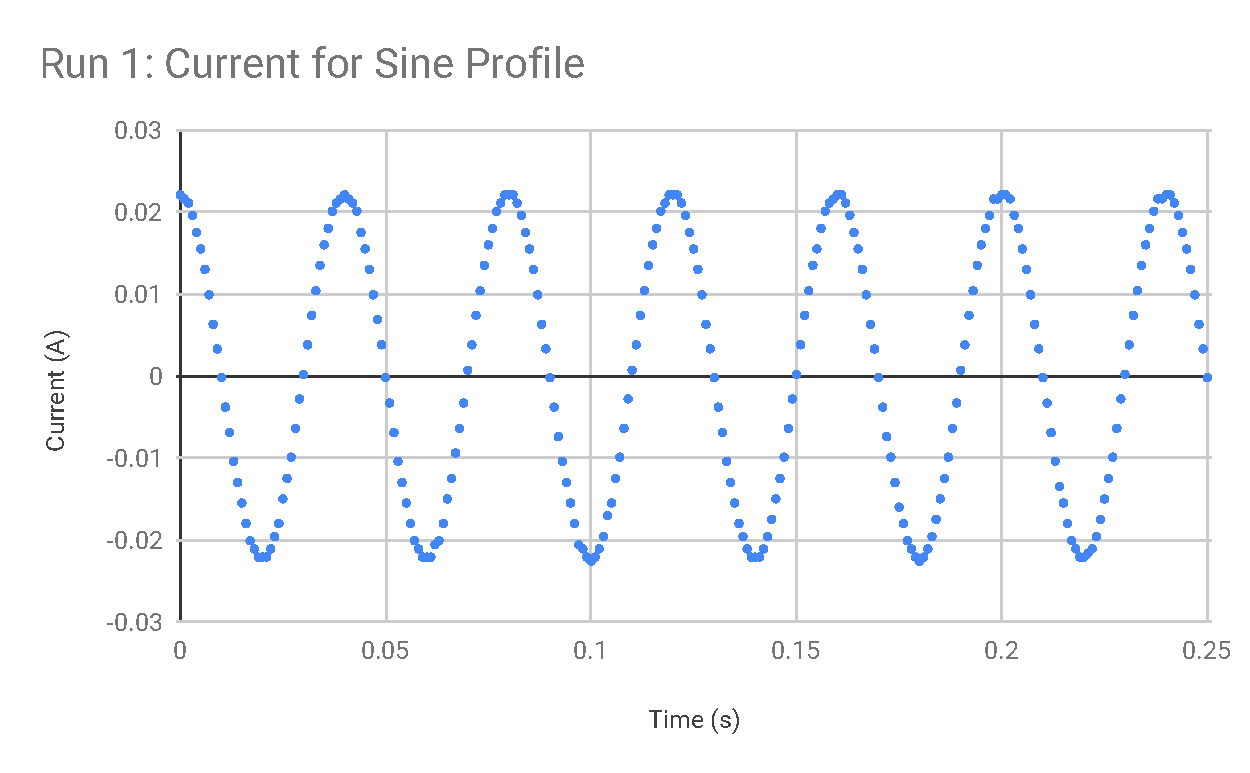
\includegraphics[scale=0.74]{image/04-faraday/run-1-I.pdf}
	\caption{Run 1 -- Current}
	\label{figure.04.run.1.I}
\end{figure}
%
\begin{figure}[ht]
	\centering
	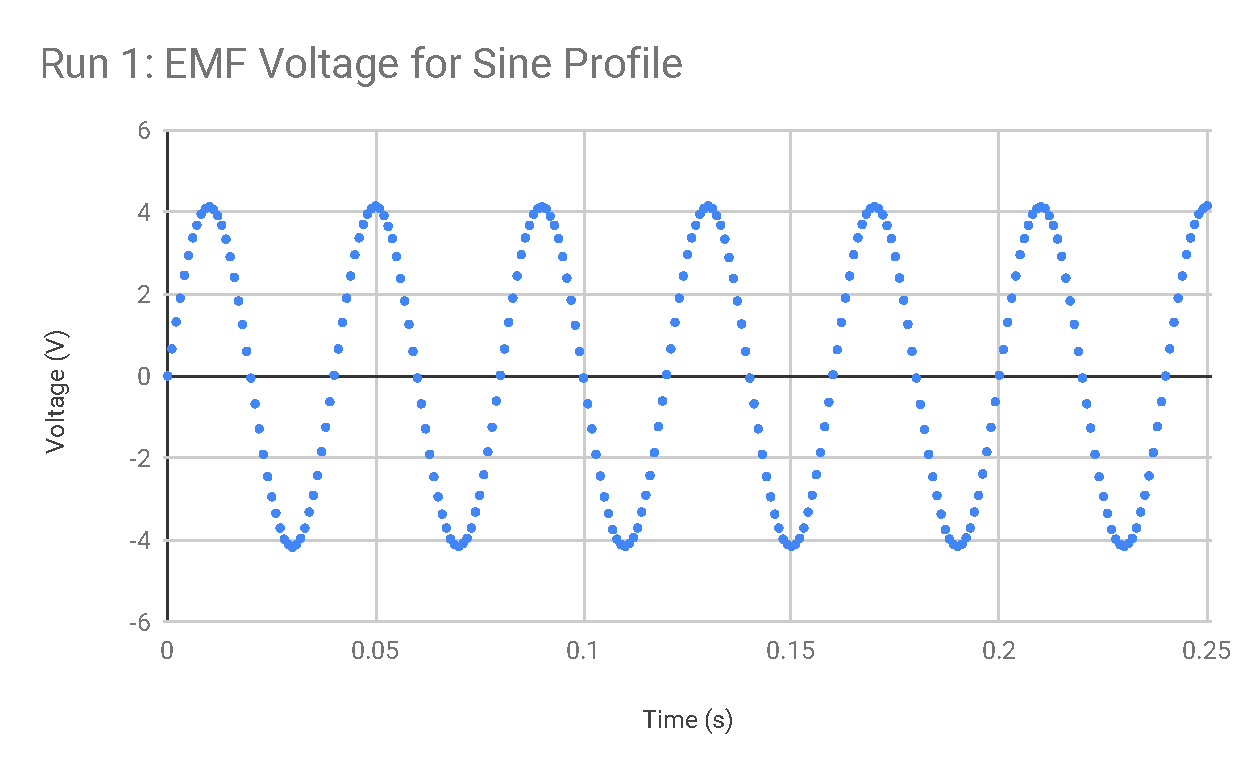
\includegraphics[scale=0.74]{image/04-faraday/run-1-V.pdf}
	\caption{Run 1 -- EMF Voltage}
	\label{figure.04.run.1.V}
\end{figure}
%
\begin{figure}[ht]
	\centering
	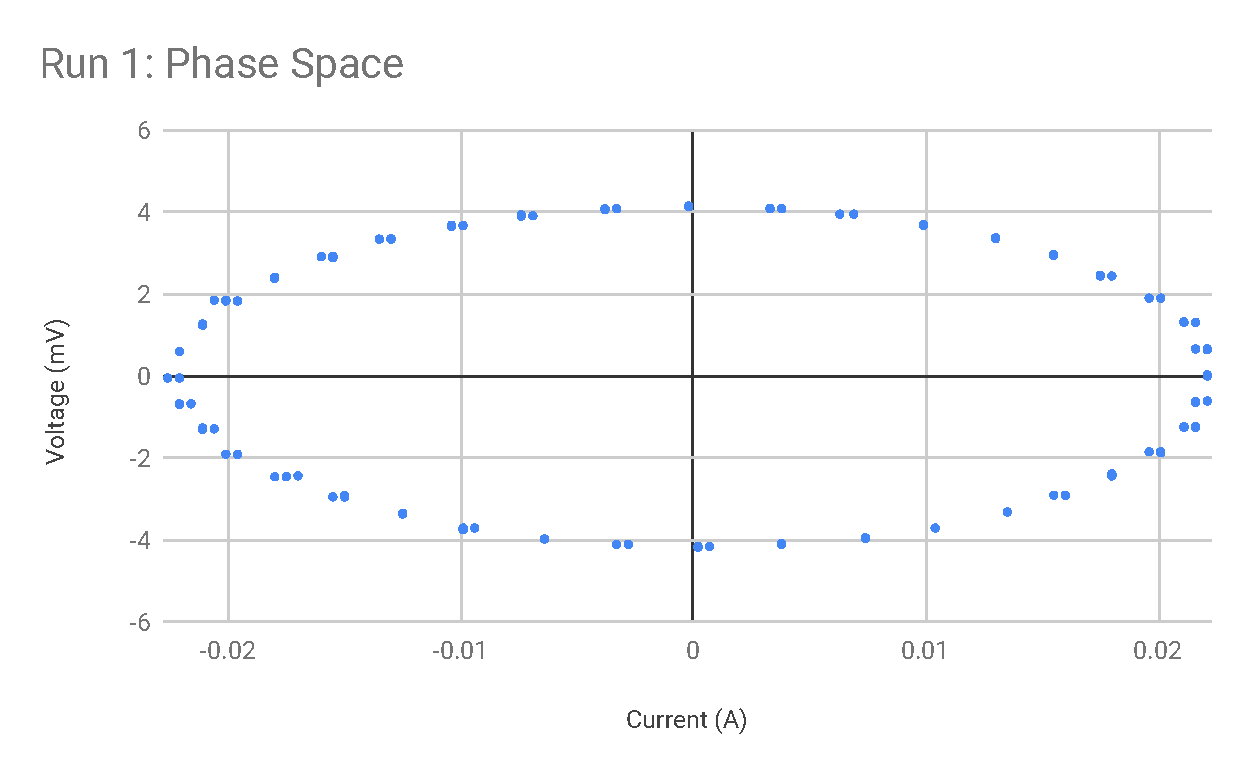
\includegraphics[scale=0.74]{image/04-faraday/run-1-phase-space.pdf}
	\caption{Run 1 -- Phase Space}
	\label{figure.04.run.1.phase.space}
\end{figure}
%
\begin{figure}[ht]
	\centering
	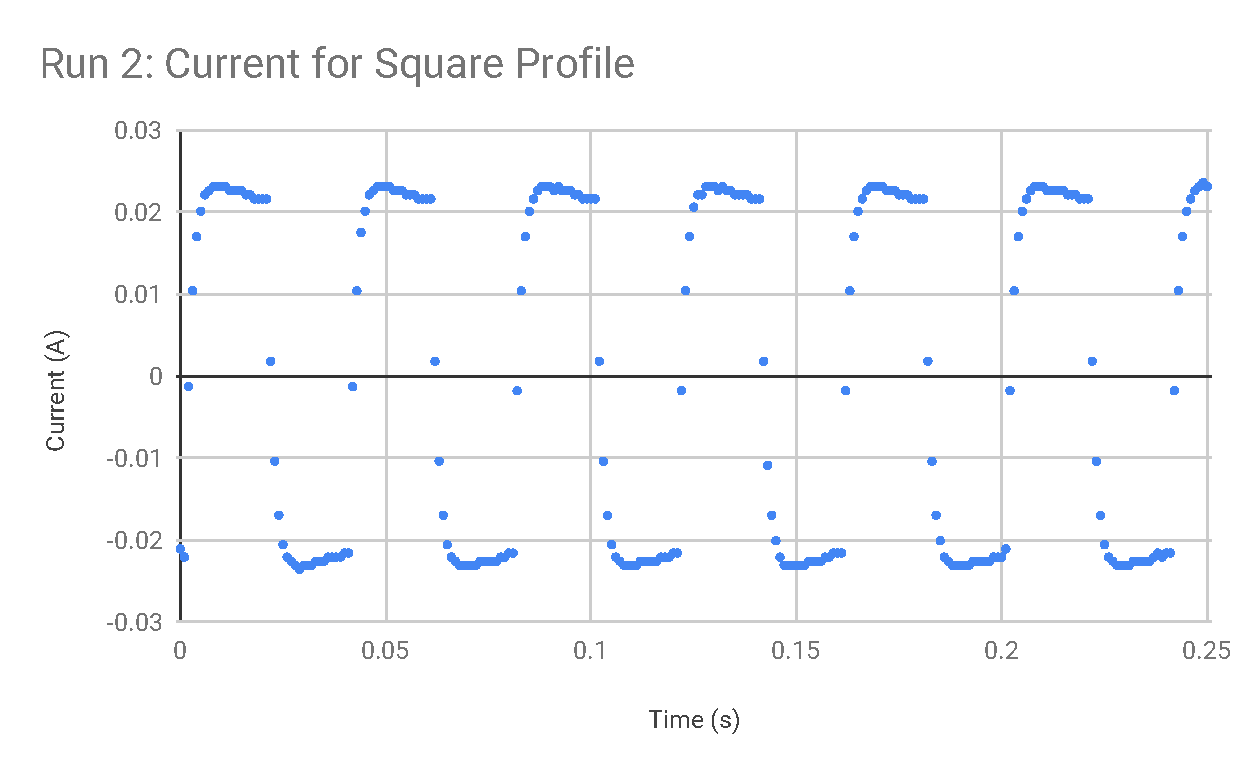
\includegraphics[scale=0.74]{image/04-faraday/run-2-I.pdf}
	\caption{Run 2 -- Current}
	\label{figure.04.run.2.I}
\end{figure}
%
\begin{figure}[ht]
	\centering
	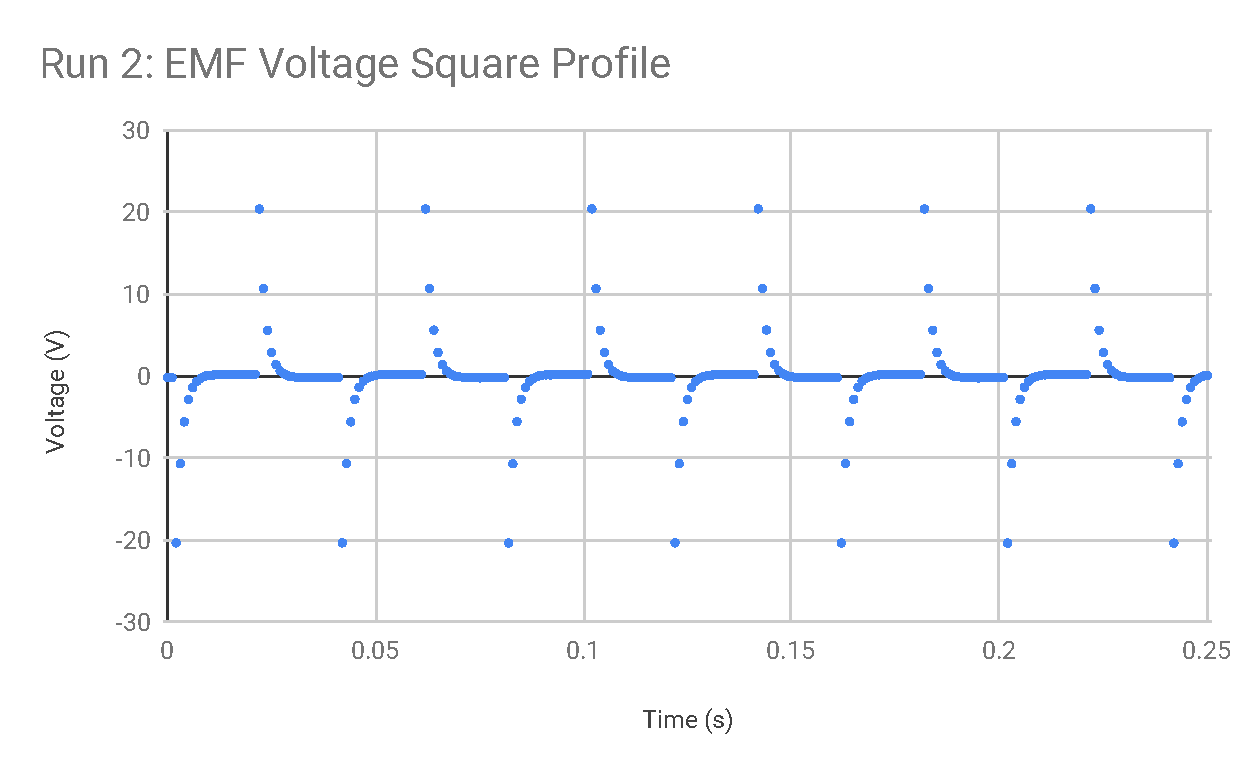
\includegraphics[scale=0.74]{image/04-faraday/run-2-V.pdf}
	\caption{Run 2 -- EMF Voltage}
	\label{figure.04.run.2.V}
\end{figure}
%
\begin{figure}[ht]
	\centering
	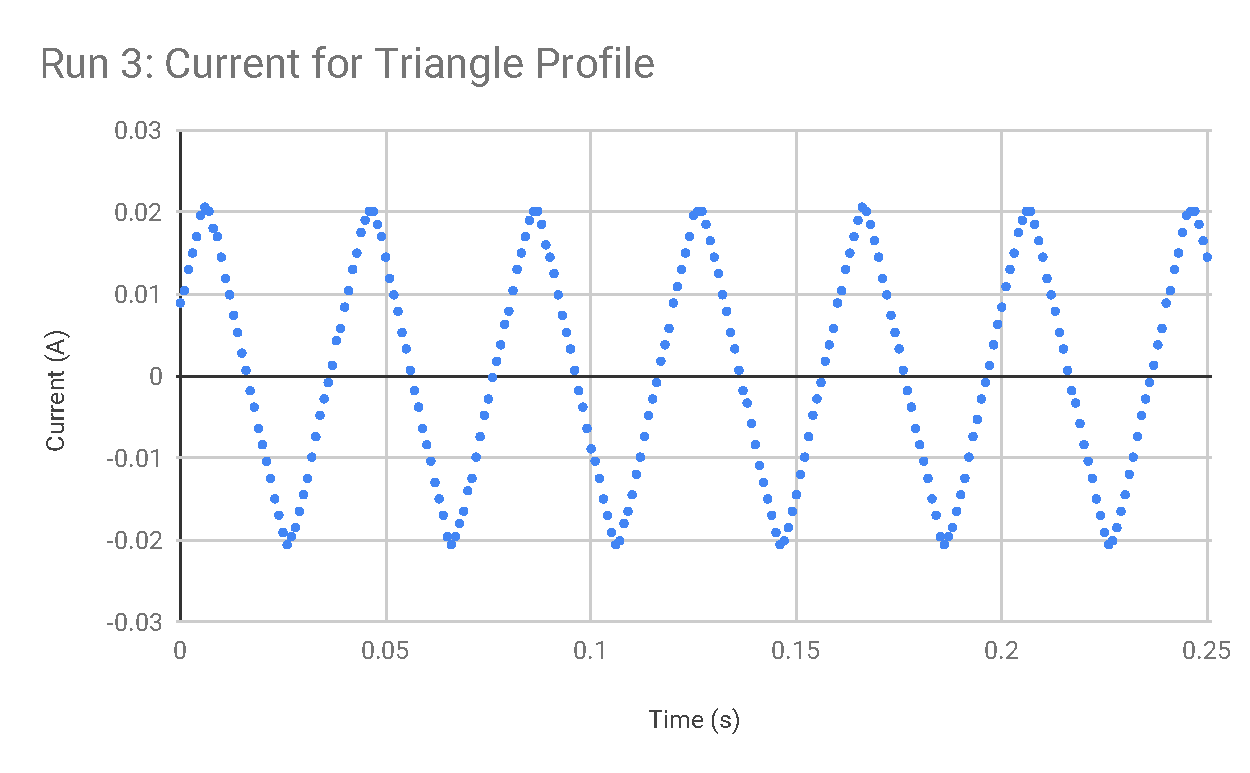
\includegraphics[scale=0.74]{image/04-faraday/run-3-I.pdf}
	\caption{Run 3 -- Current}
	\label{figure.04.run.3.I}
\end{figure}
%
\begin{figure}[ht]
	\centering
	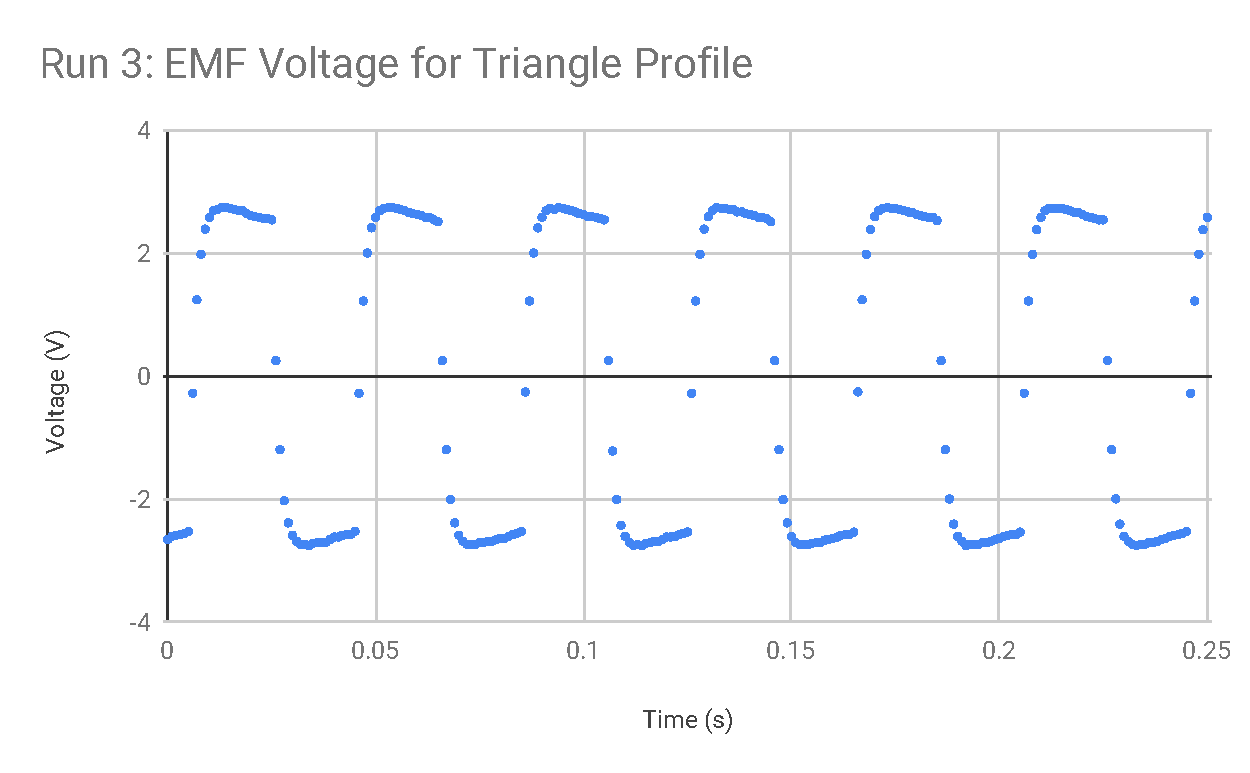
\includegraphics[scale=0.74]{image/04-faraday/run-3-V.pdf}
	\caption{Run 3 -- EMF Voltage}
	\label{figure.04.run.3.V}
\end{figure}
%
\begin{figure}[ht]
	\centering
	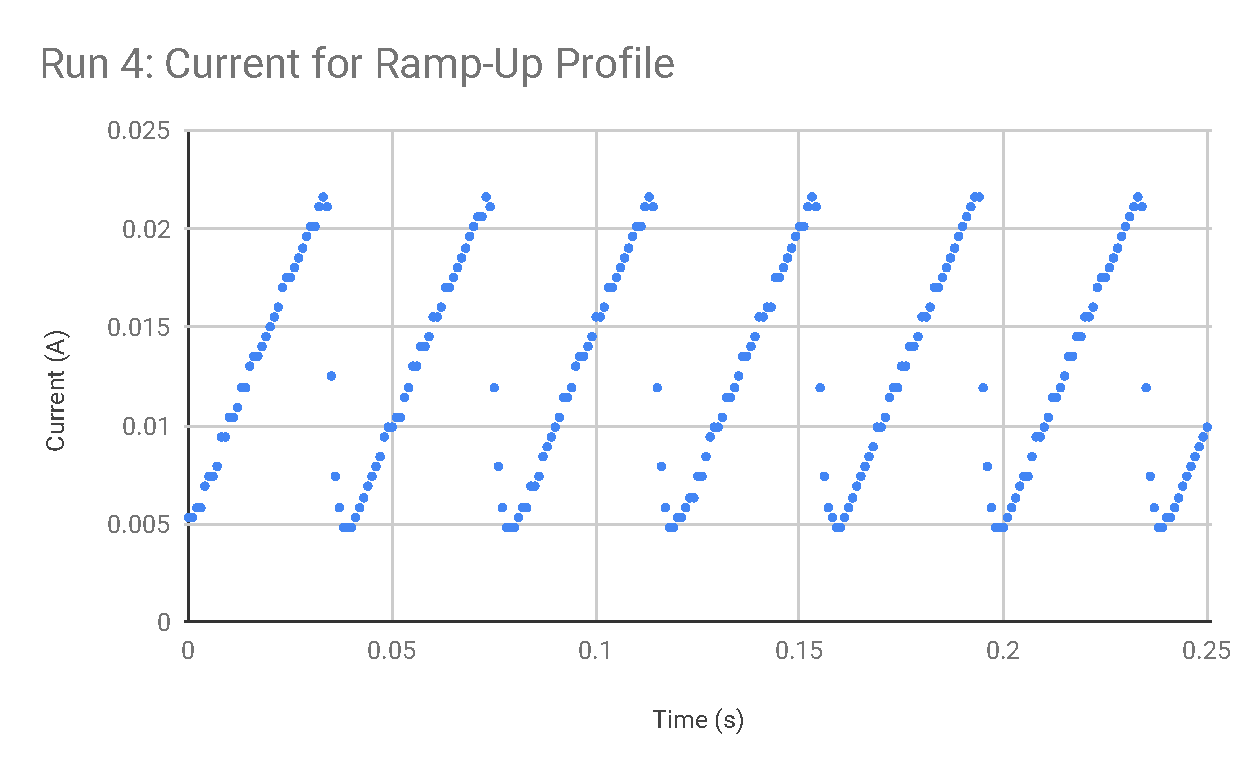
\includegraphics[scale=0.74]{image/04-faraday/run-4-I.pdf}
	\caption{Run 4 -- Current}
	\label{figure.04.run.4.I}
\end{figure}
%
\begin{figure}[ht]
	\centering
	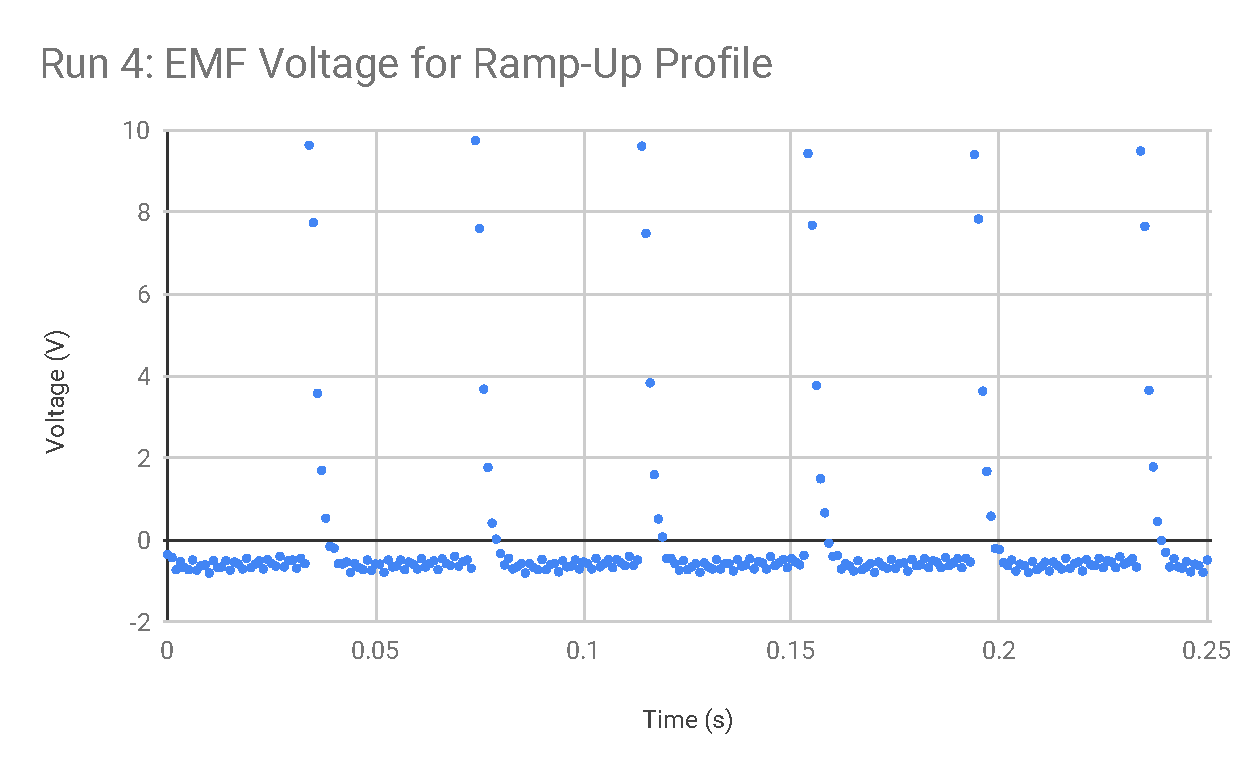
\includegraphics[scale=0.74]{image/04-faraday/run-4-V.pdf}
	\caption{Run 4 -- EMF Voltage}
	\label{figure.04.run.4.V}
\end{figure}
%
\begin{figure}[ht]
	\centering
	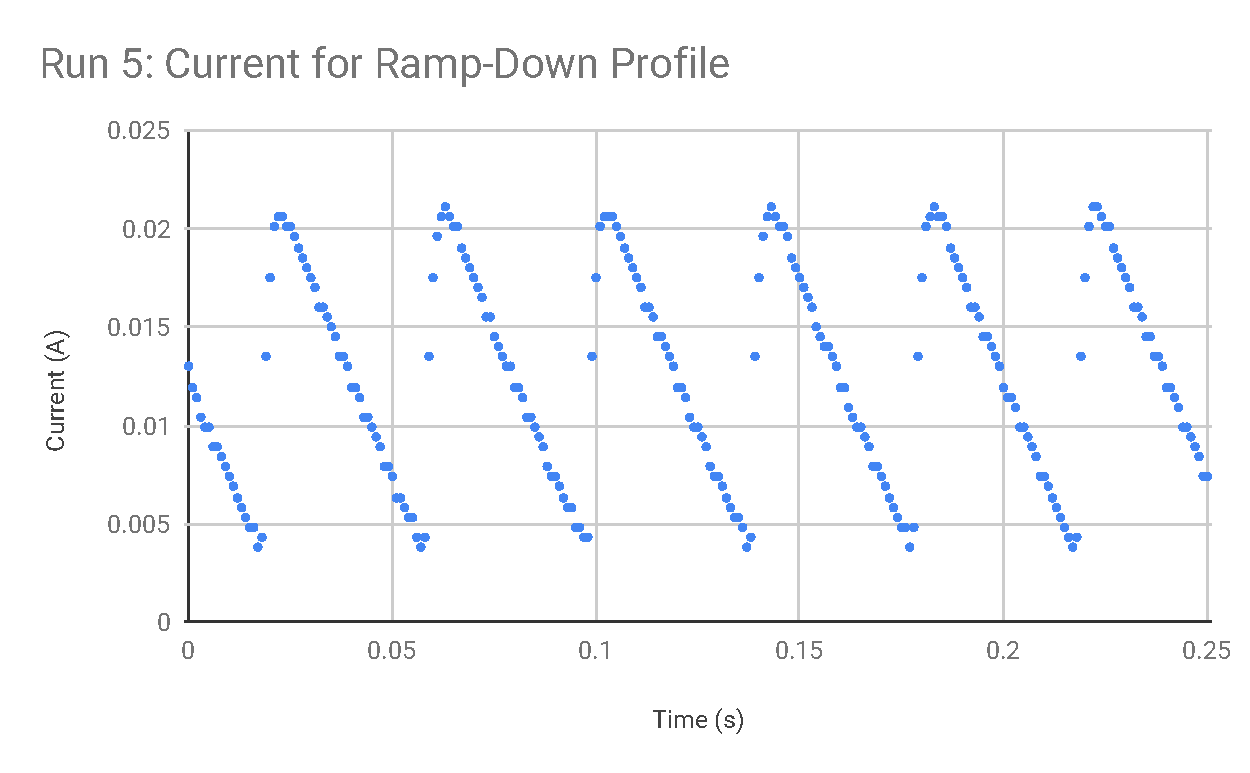
\includegraphics[scale=0.74]{image/04-faraday/run-5-I.pdf}
	\caption{Run 5 -- Current}
	\label{figure.04.run.5.I}
\end{figure}
%
\begin{figure}[ht]
	\centering
	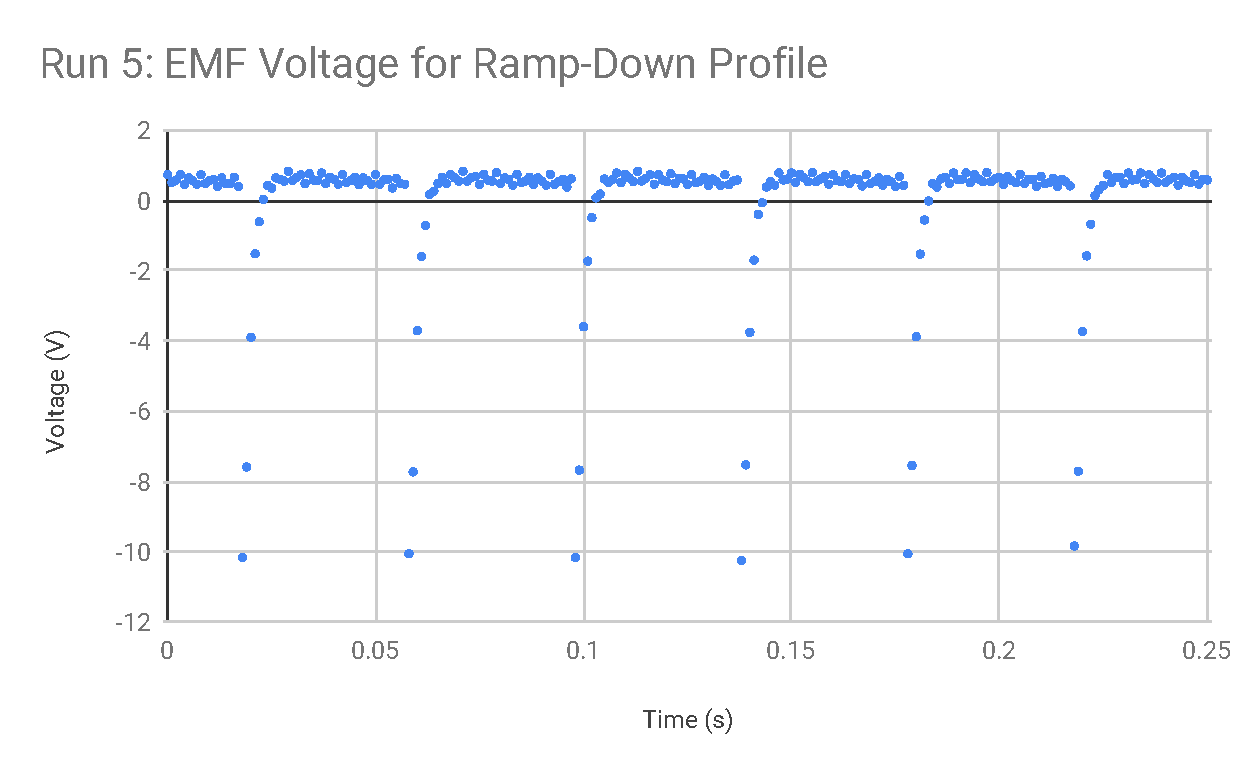
\includegraphics[scale=0.74]{image/04-faraday/run-5-V.pdf}
	\caption{Run 5 -- EMF Voltage}
	\label{figure.04.run.5.V}
\end{figure}
%
\begin{figure}[ht]
	\centering
	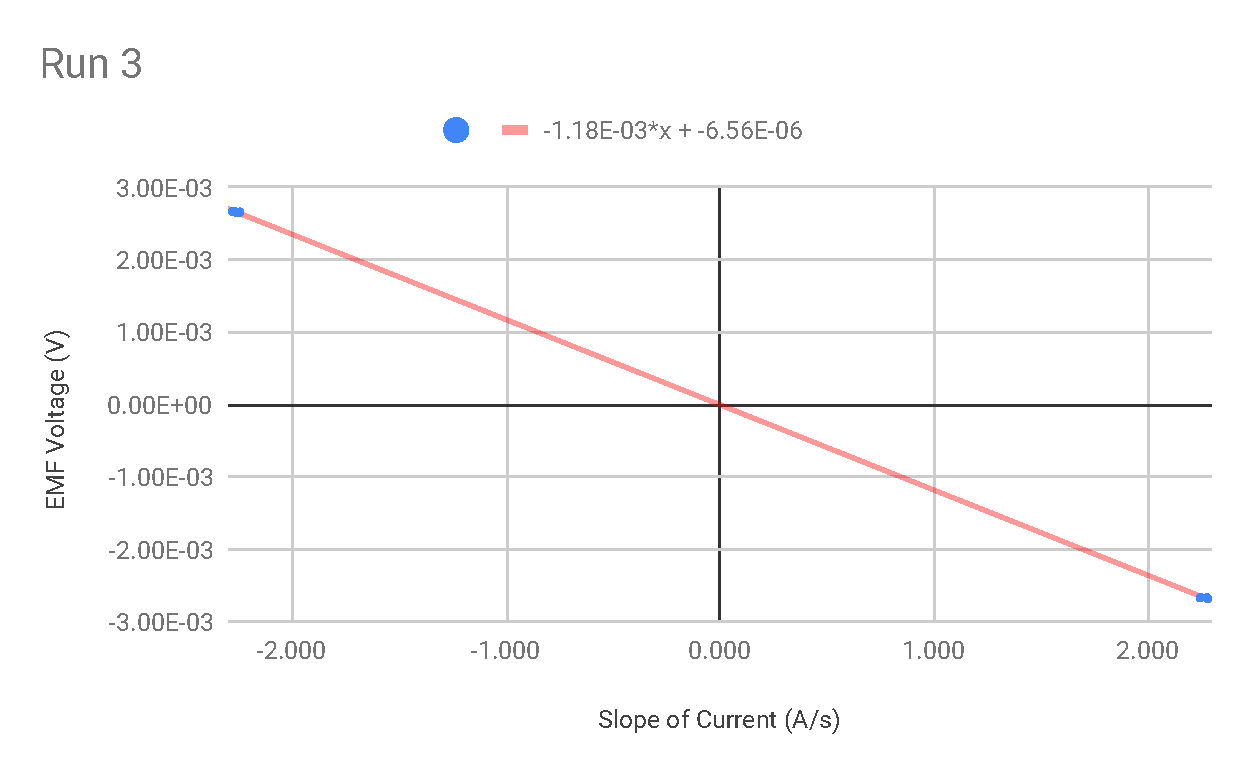
\includegraphics[scale=0.74]{image/04-faraday/run-3.pdf}
	\caption{Run 3}
	\label{figure.04.run.3}
\end{figure}